\documentclass[14pt, a4paper]{article}
\usepackage[utf8]{inputenc}
\usepackage{graphicx}
\usepackage[portuguese]{babel}
\usepackage{natbib}


\title{IF768 - TEORIA DE GRAFOS}
\author{Gustavo José Cordeiro Victor de Araújo}
\date{Abril, 2023}

\begin{document}

\maketitle
{\textbf{
\section{Introdução da Disciplina}
}}
\label{sec:introducao}

\paragraph{}

A Teoria de Grafos é uma disciplina eletiva da graduação em ciência da Compuação, que também é abordada de maneira suscinta em Matemática Discreta. Os principais objetivos dessa cadeira são aprender os conceitos de Grafos, Subgrafos e Grafos Orientados; Florestas e Árvores; Busca em Grafos, Conectividade e Cortes; Árvore Geradora, Distâncias e mostrar que é uma área extremamente importante na programação. \citep{IF768}

\begin{figure}[ht]
\centering
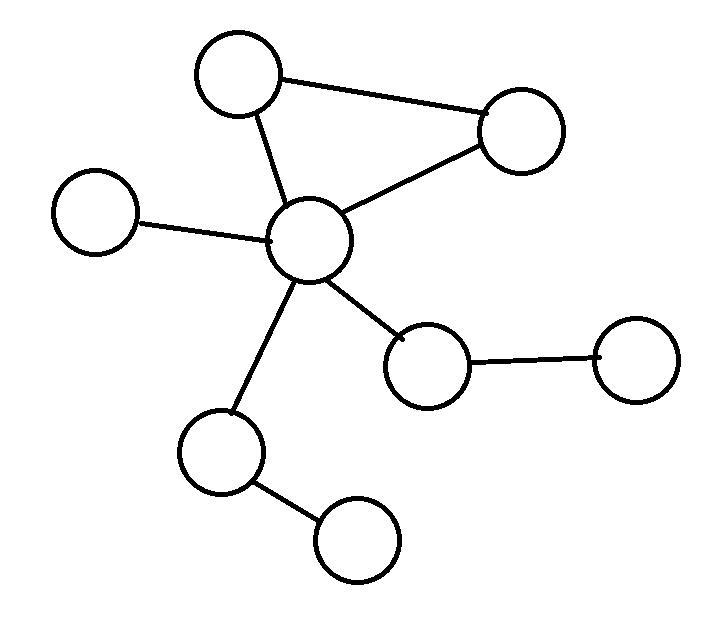
\includegraphics[width=5cm]{images/grafolegal.png}
\caption{Representação de um Grafo}
\label{figura:geometria}
\end{figure}

\paragraph{}

A teoria dos grafos é um ramo da matemática que estuda a relação entre objetos chamados "vértices" (também conhecidos como nós) e as "arestas" (também conhecidas como ligações) que conectam esses vértices. Os grafos podem ser representados visualmente como diagramas que consistem em pontos (vértices) interconectados por linhas (arestas). 

\paragraph{}

Os grafos podem ser representados de diversas formas, desde diagramas simples com círculos e linhas até estruturas de dados complexas em computadores. Existem vários tipos de grafos, incluindo grafos completos (onde todos os vértices são conectados uns aos outros), grafos bipartidos (onde os vértices podem ser divididos em dois grupos distintos), grafos cíclicos (onde há um ciclo ou circuito fechado), e muitos outros.
 
\paragraph{}
Nos itens seguintes, serão apresentadas maiores  informações a respeito da disciplina. São elas:  relevância e aplicações práticas e conexão com o Curso de Ciência da Computação.\citep{Perfil}

\section{Relevância e Aplicações Práticas da Teoria de Grafos na Área de Computação}

\paragraph{}
A teoria de grafos é extremamente relevante para a área de computação, pois permite representar e modelar problemas complexos de forma visual e abstrata. Além disso, a teoria dos grafos fornece uma ampla variedade de técnicas e algoritmos que permitem resolver problemas em várias áreas da computação. 
\paragraph{}
Algumas das aplicações práticas mais importantes da teoria dos grafos em computação incluem a análise de redes sociais, o roteamento de redes de computadores, a otimização de trajetórias de robôs, a busca em bases de dados, a otimização de sistemas de produção, a análise de dados em big data, entre outras.
\paragraph{}
A teoria dos grafos também é utilizada em algoritmos de inteligência artificial, como redes neurais e algoritmos de aprendizado de máquina, onde os grafos são usados para representar e modelar dados e relações entre eles.
\paragraph{}
Em resumo, a teoria dos grafos é uma ferramenta essencial para a resolução de problemas em computação, fornecendo uma forma intuitiva e poderosa de modelar, analisar e resolver problemas complexos em diversas áreas da tecnologia.\citep{Grafos}


\bibliographystyle{plain}
\bibliography{referencias}
\end{document}